\documentclass[a4paper, 11pt]{article}
\usepackage{color}
\usepackage{fancyhdr}
\usepackage{float}
\usepackage{stfloats}
\usepackage{placeins}
\usepackage{tabularray}
\usepackage{xcolor,colortbl}
\usepackage[top=2.5cm, bottom=2cm, left = 2.5cm, right = 2.5cm]{geometry} 
\geometry{a4paper} 
\usepackage[utf8]{inputenc}
\usepackage{textcomp}
\usepackage{graphicx} 
\usepackage{amsmath,amssymb}  
\usepackage{bm}  
\usepackage[pdftex,bookmarks,colorlinks,breaklinks]{hyperref} 
\hypersetup{linkcolor=MSBlue,citecolor=black,filecolor=black,urlcolor=black} % black links, for printed output
\usepackage{memhfixc} 
\usepackage{pdfsync}  
\usepackage{xcolor}
\usepackage{titlesec}
\usepackage{tocloft}
\usepackage{rotating}

\definecolor{MSBlue}{RGB}{47, 84, 150}
\definecolor{MSGray}{RGB}{128, 128, 128}

\renewcommand{\cftsecfont}{\fontfamily{qag}\selectfont\bfseries} 
\renewcommand{\cftsecpagefont}{\fontfamily{qag}\selectfont\bfseries\color{MSBlue}} 
\renewcommand{\cfttoctitlefont}{\fontfamily{qag}\selectfont\LARGE\bfseries}               
\renewcommand{\familydefault}{phv}

\fancypagestyle{titlepage}{
  \fancyhf{}
  \rfoot{\fontfamily{qag}\fontsize{11pt}{0pt}\selectfont\color{MSGray} version 0.2v}
  \renewcommand{\headrulewidth}{0pt}
  \renewcommand\footrulewidth{0pt}
}



\pagestyle{fancy}
\renewcommand{\headrulewidth}{0pt}
\renewcommand{\footrulewidth}{0pt}
\setlength{\headheight}{15pt}
\rhead{\fontfamily{qag}\fontsize{10pt}{12pt}\selectfont\color{MSGray} 08.06.23}
\lhead[]{}
\fancyfoot[C]{\fontsize{10pt}{10pt}\selectfont\thepage} 



\titleformat{\section}
  {\fontfamily{qag}\selectfont\LARGE\bfseries\color{MSBlue}}
  {\thesection}{0.5em}{}
  
  
\titleformat{\subsection}
  {\fontfamily{qag}\selectfont\Large\mdseries\color{MSBlue}}
  {\thesubsection}{0.5em}{}

\titleformat{\subsubsection}
  {\fontfamily{qag}\selectfont\large\mdseries\color{MSBlue}}
  {\thesubsubsection}{0.5em}{}

\titlespacing\subsubsection{0pt}{12pt plus 4pt minus 2pt}{0pt plus 2pt minus 2pt}

\linespread{1.2} 

\begin{document}

\begin{titlepage}
  \thispagestyle{titlepage}
  \begin{center} 
    
\includegraphics[width=150pt]{..//ArduFlowLogo.png}
    \end{center}


	\setlength{\parindent}{0pt}
	\vspace*{.15\textheight}
	\medbreak
	{\fontfamily{qag}\Huge\bfseries\color{MSBlue}Personal Project Architecture\par}
	\bigbreak
    \bigbreak
	{Michał Raczkowski\par}
    \smallbreak
    {\small OL S6 \par}
    \smallbreak
    {\small 4465024\par}
\end{titlepage}



\pagebreak


\tableofcontents

\vfill
\begin{table}[b]
  \centering
  \begin{tblr}{
    width = \linewidth,
    colspec = {Q[200]Q[133]Q[327]Q[248]},
    hlines,
    vlines,
  }
  \textbf{Version} & \textbf{Date} & \textbf{Author} & \textbf{Comment} \\
   0.1v                & 04.06.23             & M. Raczkowski   & Introduction, Electron.js \\
   0.2v                & 08.06.23               & M. Raczkowski & Arduino-cli, Model-C4 \\
   

  \end{tblr}
\end{table}


\pagebreak


\section{Introduction}
ArduFlow is a user-friendly desktop application that simplifies LED 8x8 matrix animation programming with Arduino. This paper provides an overview of ArduFlow's architecture, highlighting its key components and interactions. By using the C4 model, we present a structured representation of ArduFlow's design, enabling developers and stakeholders to understand its capabilities and potential for further development. 

\section{Electron}

\subsection{Main Process}
The main process is the heart of Electron.js applications. It runs in the main thread and is responsible for managing the application's lifecycle and interacting with the underlying operating system. It provides system-level functionalities such as file system access, inter-process communication, and native API integration. The main process is typically implemented using Node.js, which enables developers to utilize the vast ecosystem of Node.js modules and libraries.

\subsection{Renderer Process}
The renderer process handles the rendering of the user interface and runs in separate Chromium-based browser windows or webviews. Each renderer process corresponds to a single web page or view in the application. It utilizes web technologies such as HTML, CSS, and JavaScript to create the user interface, handle user interactions, and communicate with the main process through inter-process communication mechanisms. The renderer process is isolated from the main process, providing security and stability.

\subsection{Inter-Process Communication (IPC)}
Electron.js facilitates communication between the main process and renderer processes through Inter-Process Communication (IPC). IPC enables seamless data exchange and function invocation between the different processes. It allows developers to pass messages, invoke methods, and share data between the main and renderer processes, enabling effective coordination and synchronization.

\subsection{Cross-Platform Capabilities}
One of the key advantages of Electron.js is its ability to build cross-platform desktop applications. The architecture of Electron.js abstracts away the underlying operating system differences, allowing developers to write code once and deploy it on multiple platforms. Electron.js achieves this by providing a consistent runtime environment across operating systems, ensuring that the application behaves consistently on Windows, macOS, and Linux.

\subsection{Web Technologies and Tooling}
Electron.js leverages web technologies, including HTML, CSS, and JavaScript, for building the user interface and application logic. This enables developers to utilize their existing web development skills and frameworks. Electron.js provides a rich set of APIs and tools to create desktop-like experiences using familiar web development patterns. The architecture of Electron.js enables seamless integration with popular web frameworks and libraries, making it flexible and adaptable for a wide range of use cases.

\bigbreak

In summary, the architecture of Electron.js combines the main process, renderer process, and IPC mechanisms to create cross-platform desktop applications using web technologies. This architecture empowers developers to leverage their web development skills, utilize the vast Node.js ecosystem, and build feature-rich applications that work consistently across different operating systems.

\section{Arduino-cli}

Arduino-cli is a command-line interface (CLI) tool that provides a unified and streamlined way to interact with Arduino boards and libraries. It follows a modular architecture that consists of several key components and functionalities.

\subsection{Command-Line Interface}
The command-line interface is the primary user interface of Arduino-cli. It allows developers to execute various commands to manage Arduino boards, libraries, and sketches. Users interact with the CLI by typing commands and providing relevant arguments and options. The CLI parses these inputs and triggers the corresponding actions or operations.
\subsection{Core Modules}
Arduino-cli consists of several core modules that handle different aspects of the development workflow. These modules include board, library, sketch, and compile, among others. Each module is responsible for specific operations, such as managing board configurations, handling library dependencies, managing sketches, and compiling code.
\subsection{Configuration Files}
Arduino-cli utilizes configuration files to store settings and preferences related to boards, libraries, and other tools. These configuration files help in managing and maintaining consistent development environments. Users can modify these files to customize their development settings, such as specifying the board type, communication ports, and library paths.
\subsection{Board Manager}
The board manager is a crucial component of Arduino-cli that handles board-related operations. It allows users to install, update, and manage board definitions for different Arduino platforms. The board manager enables developers to easily switch between different boards, manage board-specific settings, and handle board-specific tasks like uploading code and setting bootloader configurations.
\subsection{Library Manager}
The library manager provides functionalities for managing Arduino libraries. It allows users to install, update, and remove libraries required for their projects. The library manager handles library dependencies, ensuring that the necessary libraries are available and up to date. It simplifies the process of integrating third-party libraries into Arduino projects.
\subsection{Sketch Management}
Arduino-cli provides capabilities for managing sketches, which are the code files containing Arduino programs. Users can create, edit, compile, and upload sketches to Arduino boards using the CLI. The sketch management component handles the organization and compilation of Arduino code, making it easier for developers to work with multiple sketches and manage their dependencies.
\subsection{Integration with Build Systems}
Arduino-cli integrates with popular build systems, such as Makefile and CMake, allowing developers to leverage their preferred build tools. This integration enables more advanced and customized build configurations for complex projects. Developers can utilize the CLI commands and tools in conjunction with build systems to streamline their development processes.

\bigbreak

Overall, the architecture of Arduino-cli revolves around the command-line interface, core modules, configuration files, board manager, library manager, sketch management, and integration with build systems. This modular architecture provides a flexible and efficient way to interact with Arduino boards, manage libraries, and compile and upload sketches, simplifying the development workflow for Arduino projects.

\section{Context Diagram}

\begin{figure}[H]
    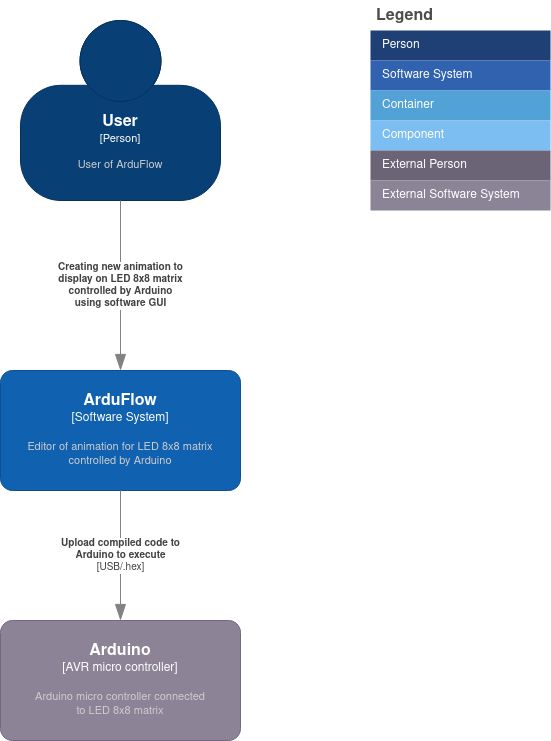
\includegraphics[width=\linewidth]{C4model/ArduFlow c4-1.png}
    \caption{Level 1 of C4 model}
    \label{fig:Level 1 of C4 model}
\end{figure}
\section{Container Diagram}
\begin{figure}[H]
    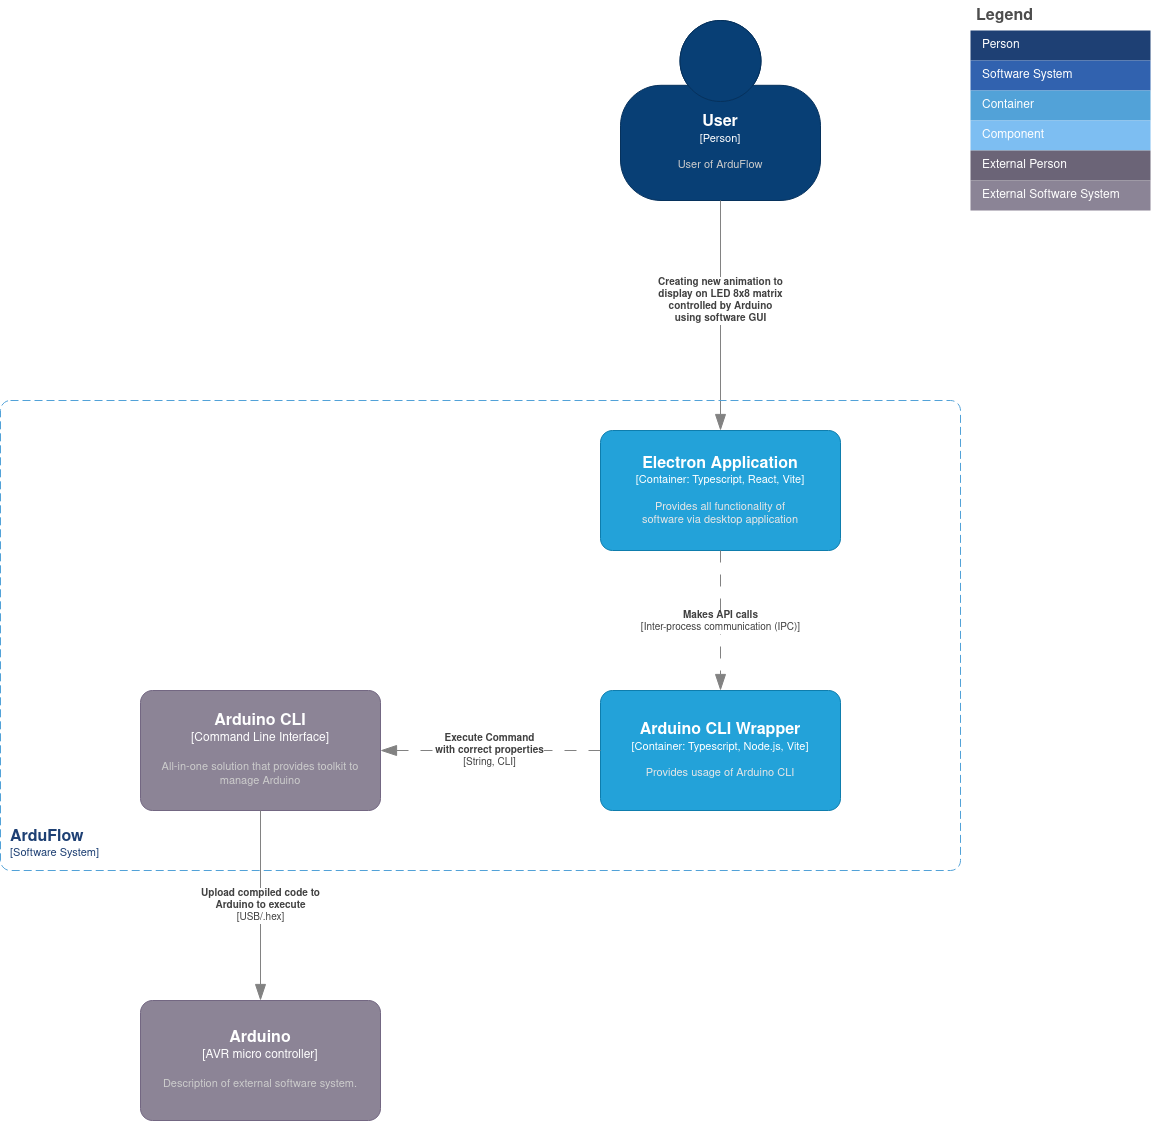
\includegraphics[width=\linewidth]{C4model/ArduFlow c4-2.png}
    \caption{Level 2 of C4 model}
    \label{fig:Level 2 of C4 model}
\end{figure}


\section{Component Diagram}
\begin{figure}[H]
    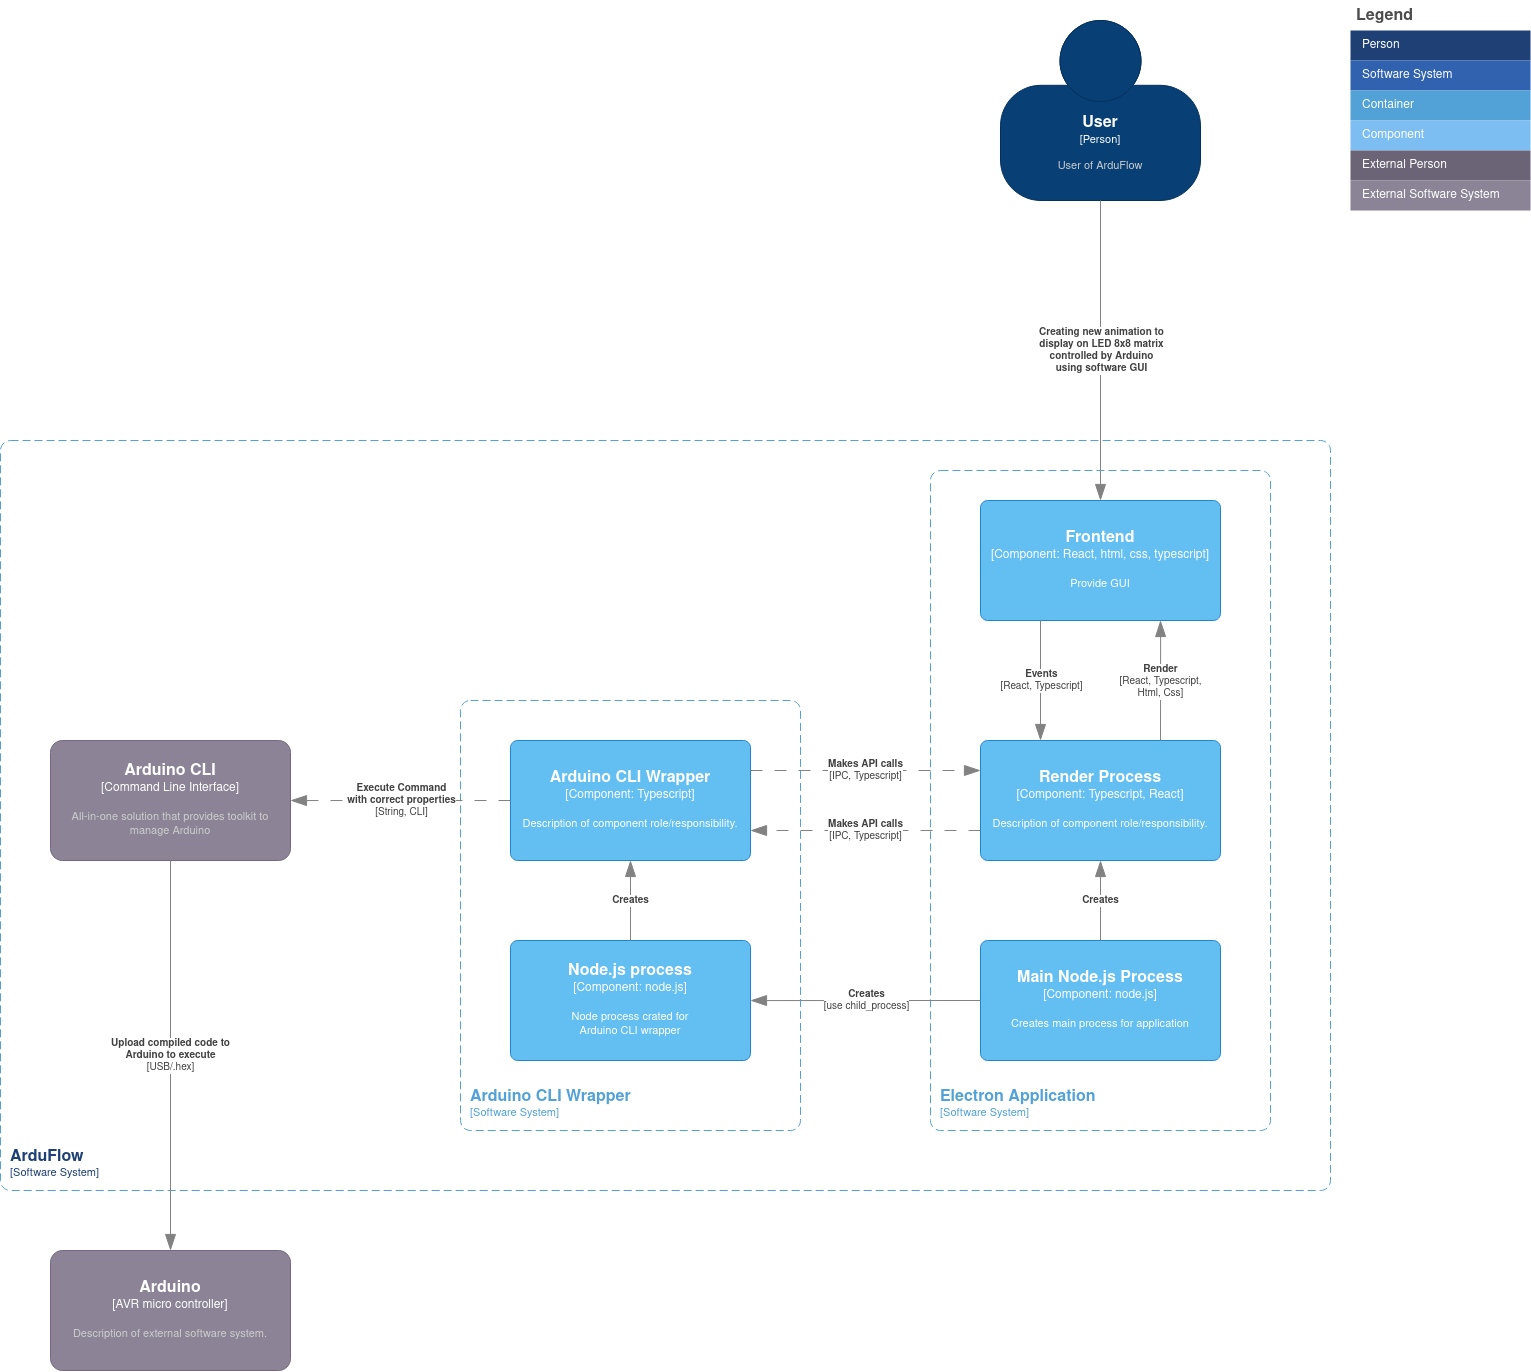
\includegraphics[width=\linewidth]{C4model/ArduFlow c4-3.png}
    \caption{Level 3 of C4 model}
    \label{fig:Level 3 of C4 model}
\end{figure}

\section{Code Diagram}

Work in progress




\pagebreak


\end{document}